\documentclass{beamer}
%\usetheme{Ilmenau}
%\usecolortheme{beaver}

\usepackage[slovak,american]{babel}
\usepackage[utf8]{inputenc}
\usepackage{graphicx}
\usepackage{adjustbox}
 \usepackage{xcolor}
 
 \newsavebox\MBox
\newcommand\Cline[2][red]{{\sbox\MBox{$#2$}%
  \rlap{\usebox\MBox}\color{#1}\rule[-2.2\dp\MBox]{\wd\MBox}{1pt}}}

%\usefonttheme{serif}

\definecolor{UKOrange}{HTML}{ef9424} %
\definecolor{UKBrown}{HTML}{a96d5e} %
\definecolor{UKLight}{HTML}{d8b6ab} %
\definecolor{UKDark}{HTML}{7a4f44}
\definecolor{UKDarker}{HTML}{4d312b} 
\definecolor{UKDarkest}{HTML}{2e1e1a}
\definecolor{UKRed}{HTML}{bf1f1c}

\setbeamertemplate{footline}[frame number]{}
\setbeamertemplate{navigation symbols}{}

%\usecolortheme{beaver}
\setbeamertemplate{itemize item}[square]
\setbeamercolor{itemize item}{fg = UKBrown}
\setbeamercolor{itemize subitem}{fg = UKLight}
\setbeamercolor{enumerate item}{fg = UKDark}

\setbeamercolor{footnote}{fg=UKLight}
\setbeamercolor{footnote mark}{fg=UKLight}
\setbeamerfont{footnote}{size=\tiny}
\renewcommand\footnoterule{}

\usetheme{default}
\beamertemplatenavigationsymbolsempty
\setbeamercolor{title}{fg=white, bg=UKBrown}
\setbeamercolor{frametitle}{fg=white, bg=UKBrown}
\setbeamercolor{block title}{bg=UKBrown, fg= white}
\setbeamercolor{block body}{bg =UKLight, fg = UKDarkest}

\useoutertheme[subsection=false]{miniframes}
\AtBeginSection[]{\subsection{}}

\setbeamercolor{below lower separation line head}{bg=UKDark}
\addtobeamertemplate{headline}{}{%
  \begin{beamercolorbox}[colsep=0.5pt]{below lower separation line head}
  \end{beamercolorbox}
}
%\setbeamercolor*{mini frame}{fg=white,bg=UKRosy}
\setbeamercolor{section in head/foot}{fg=UKLight, bg=UKDark}

%\setbeamertemplate{itemize/enumerate body begin}{\normalsize}
%\setbeamertemplate{itemize/enumerate subbody begin}{\normalsize}




%\newcommand{\codeblock}[2]{ \begin{block}{#1} \begin{verbatim}#2\end{verbatim}\end{block}}

%\defbeamertemplate*{title page}{customized}[1][]
%{
%  \begin{centering}
%    \begin{beamercolorbox}[sep=8pt,center]{title}
%      \usebeamerfont{title}\inserttitle
%    \end{beamercolorbox}
%  \end{centering}
%  \bigskip
%
%\begin{columns}[onlytextwidth,T]
%
%
%  \column{27mm}
%  \includegraphics[width=27mm]{images/logoFMFI.png}
%  
%  \column{\dimexpr\linewidth-54mm-6mm}
%  \centering
%  \vspace{5mm}  
%  \usebeamerfont{author}\insertauthor\par
%  \vspace{5mm}
%  \usebeamerfont{institute}\insertinstitute\par
%
%  \column{27mm}
%  \includegraphics[width=27mm]{images/logoUK.png}  
%\end{columns}
%\centering
%\vspace{7mm}
%  \usebeamerfont{date}\insertdate\par
%}


\title[PCA a LDA]{Rozpoznávanie obrazcov - 5. cvičenie \\ Redukcia dimenzionality}
\author[Viktor Kocur]{Viktor Kocur \\{\small viktor.kocur@fmph.uniba.sk}}
\institute{DAI FMFI UK}
\date{16.3.2020}
%\titlegraphic{\includegraphics[width=2.7cm]{images/logoFMFI.png}\hspace*{1cm}~%
%   \includegraphics[width=2.7cm]{images/logoUK.png}
%}


\begin{document}
\selectlanguage{slovak}

\begin{frame}[plain]
  \titlepage  
\end{frame}

\section{PCA}

\begin{frame}
\frametitle{PCA princíp}
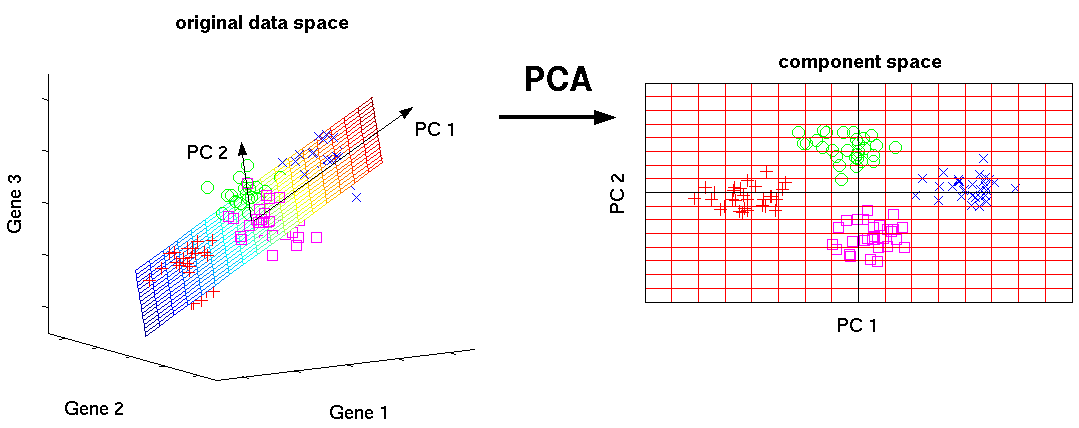
\includegraphics[width=\textwidth]{PCA.png}
\end{frame}


\begin{frame}
\frametitle{PCA motivácia}
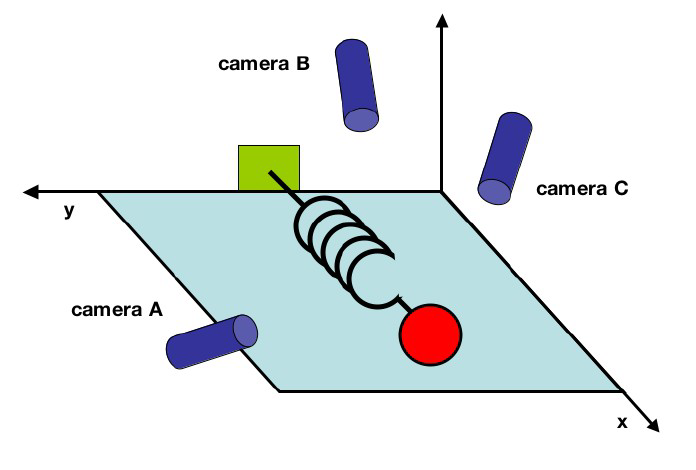
\includegraphics[width=\textwidth]{PCAcameras.png}
\end{frame}


\begin{frame}
\frametitle{PCA matematika}

\begin{block}{Vlastné vektory a čísla}
Nech $\mathbb{A}$ je matica $n \times n$, potom nenulový vektor $\vec{v} \in \mathbb{R}^n$ je vlastný vektor matice $\mathbb{A}$ s vlastným číslom $\lambda \in \mathbb{C}$ ak platí: $\mathbb{A}\vec{v} = \lambda \vec{v}$. 
\end{block}

\begin{block}{Hermitovské matice}
Hermitovské matice majú iba reálne vlastné čísla. Taktiež je možné vždy ku každému vlastnému číslu nájsť reálny vlastný vektor.
\end{block}
\end{frame}


\begin{frame}
\frametitle{PCA matematika}

\begin{block}{Kovariancia}
$cov (X, Y) = \frac{\sum_{i=1}^n (X_i - \overline{X})(Y_i - \overline{Y})}{n}$
\end{block}

\begin{block}{Kovariančná matica}
$COV(X)_{i,j} = cov(X_i, X_j)$
\end{block}

\begin{block}{Kovariančná matica}
Kovariančná matica je Hermitovská a pozitívne semi-definitná.
\end{block}
\end{frame}



\begin{frame}
\frametitle{PCA matematika}

\begin{block}{Matica vlastných vektorov}
Z normalizovaných vlastných vektorov $v_1 ... v_n$ zostavíme maticu $(v_1, v_2, ... , v_n)$. Značíme $\mathbb{W}$.
\end{block}

\begin{block}{PCA}
PCA spočíva v tom, že vlastné vektory kovariančnej matice reprezentujú ortogonálnú bázu v ktoré je kovariančná matica dát diagonálna.
\end{block}

\begin{block}{PCA - postup}
Naše dáta najprv centrumjeme $\vec{x}' = \vec{x} - \overline{x}$. Potom vypočítame $\mathbb{W}$. Nové dáta dostaneme maticovým násobením $ y = \vec{x}' \mathbb{W}^T$, ak je vektor $\vec{x}$ riadkový. Vlastné čísla korešpondujú k podielu celkovej variancie v danom smere. Podiel vlastného čísla so súčtom vlastných čísiel určuje aký podiel variancie vie daný smer vysvetliť.  
\end{block}
\end{frame}



\begin{frame}
\frametitle{Postup matlab}

\begin{block}{Načítanie dát}
load data.mat
\end{block}

\begin{block}{Úloha}
Zobrazte si dáta v 2D plote.
\end{block}

\end{frame}


\begin{frame}
\frametitle{Postup matlab}

\begin{block}{cov}
cov(A) - vráti kovariančnú maticu A
\end{block}

\begin{block}{eig}
[W, vals] = eig(A) - vráti maticu W s vlastnými vektormi a maticu vals s vlastnými čislami na diagonále.
\end{block}

\begin{block}{Úloha}
Aplikujte na dáta PCA a zobrazte si nový plot. Ktorá zložka zodpovedá akej variancii.
\end{block}
\end{frame}

\begin{frame}[fragile]
\frametitle{Riešenie}
\begin{verbatim}
load data.mat
plot(data(:,1), data(:,2), 'r*');
centered = data - mean(data);
[W, eigenvals] = eig(cov(centered))
newdata = centered * W'
plot(newdata(:,1), newdata(:,2), 'r*');
ylim([-2 2]);
xlim([-2 2]);
disp(diag(eigenvals)/sum(diag(eigenvals)))
\end{verbatim}
\end{frame}

\begin{frame}
\frametitle{Matlab - pca}

\begin{block}{pca}
[coeff,score,$\sim$ ,$\sim$,explained,mu] = pca(X) - vráti transformačnú maticu coeff (naše $\mathbb{W}^T$), transformované dáta score, percentá na koľko vysvetĺujú varianciu jednotlivé smery a stredné hodnoty $X$.
\end{block}

\begin{block}{Platí}
score == (X - mu) * coeff
\end{block}

\begin{block}{Platí}
X == score * coeff' + mu
\end{block}

\begin{block}{Úloha}
Otestujte túto funkciu na data.mat
\end{block}

\end{frame}

\begin{frame}
\frametitle{Matlab - pca}

\begin{block}{Dáta}
load ovariancancer
\end{block}

\begin{block}{gscatter}
gscatter(obs(:,1), obs(:,2), grp) - zobrazí body z prvého a druhého stĺpca pre dáta a pridelí im farbu podľa príslušnosti v grp
\end{block}

\begin{block}{Úloha}
Zistite koľko príznakov potrebujete po aplikácii PCA, aby ste s dát v obs dostali 95 percent variancie. Čo ak niektoré vlastné čísla sú nulové?
\end{block}

\begin{block}{Úloha}
Zobrazte si prvé dva smery po PCA pomocou gscatter.
\end{block}
\end{frame}


\begin{frame}
\frametitle{PCA - úlohy}

\begin{block}{Úloha}
Pre dáta z data.mat zobrazte smery do ktorých PCA premetie dáta v originálnej súradnicovej sústave.
\end{block}

\begin{block}{Úloha}
Vytvorte funkciu ktorá zoberie obrázok a ako dáta vezme jednotlivé trojice RGB pixelov. Urobí PCA na týchto dátach a nastaví na posledný (alebo posledné dva) stĺpce nulu a prekonvertuje obraz naspäť do RGB.
\end{block}

\begin{block}{Úloha}
Pre PCA z druhej úlohy zobrazte v novom obrázku rôzne farby, ktoré môžete v tejto reprezentácii používať.
\end{block}
\end{frame}


\section{LDA}
\begin{frame}
\frametitle{LDA}

\begin{block}{LDA.m}
[Y, W, lambdas] = LDA(X, T) - pre dáta X a triedy T vráti nové hodnoty po transformácii Y, maticu W a hodnotu jednotlivých vlastných čísel.
\end{block}

\begin{block}{Pozn}
Y == X * W
\end{block}

\begin{block}{Úloha}
Načítajte si Fisherovu databázu (load fisheriris). A poronvajte LDA a PCA. Pozn.: ako T v LDA použite categorical(species).
\end{block}

\begin{block}{Úloha}
Pre rôzne dvojice stĺpcov nakreslite do grafu smer do ktorého bude LDA premietať dáta.
\end{block}
\end{frame}


\begin{frame}
\frametitle{LDA}

\begin{block}{LDA.m}
MdlLinear = fitcdiscr(X,T) - vráti lineárny klasifikátor, ktorý využíva LDA. V projekte asi používajte toto.
\end{block}

\begin{block}{Tutorial}
https://www.mathworks.com/help/stats/create-and-visualize-discriminant-analysis-classifier.html
\end{block}
\end{frame}

\end{document}